 %%%%%%%%%%%%%%Empieza la presentacion%%%%%%%%%%%%%%%%%%%%%%%%%%%%%%%%%%%%

% \begin{frame}
% \frametitle{Esquema}
%    \tableofcontents
% \end{frame}


\begin{frame}
\frametitle{Filtros Ideales}

\begin{columns}[T]
\begin{column}{5cm}
\scriptsize
\centering{
Filtro paso bajo}


\vspace{0.1cm}

$\scriptsize H(jw)\!=\!\left \{  \!\!\!\begin{array}{l} 1, \: \textrm{para } |w|\!\!<\!\!w_c\\0, \:\textrm{c.c.}  \end{array}\right .$


\vspace{-0.4cm}

{\begin{figure} \centering 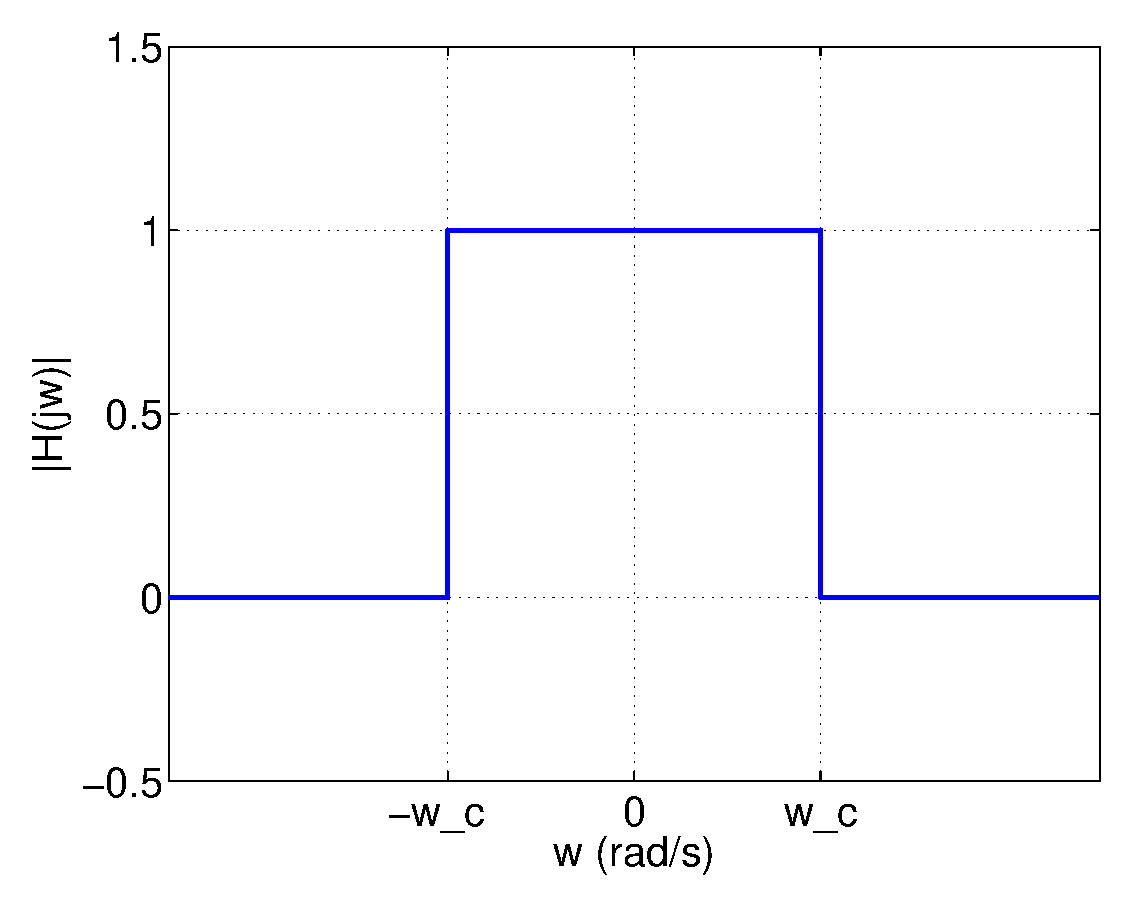
\includegraphics[width=3.2cm]{Figures/FiltroPBaja.eps}  \end{figure}}

\vspace{-0.2cm}


\scriptsize
\centering{
Filtro paso alta}

\vspace{0.1cm}
$\scriptsize H(jw)\!=\!\left \{  \!\!\!\begin{array}{l} 0, \: \textrm{para } |w|\!\!<\!\!w_c\\1, \:\textrm{c.c.}  \end{array}\right .$

\vspace{-0.4cm}

{\begin{figure} \centering 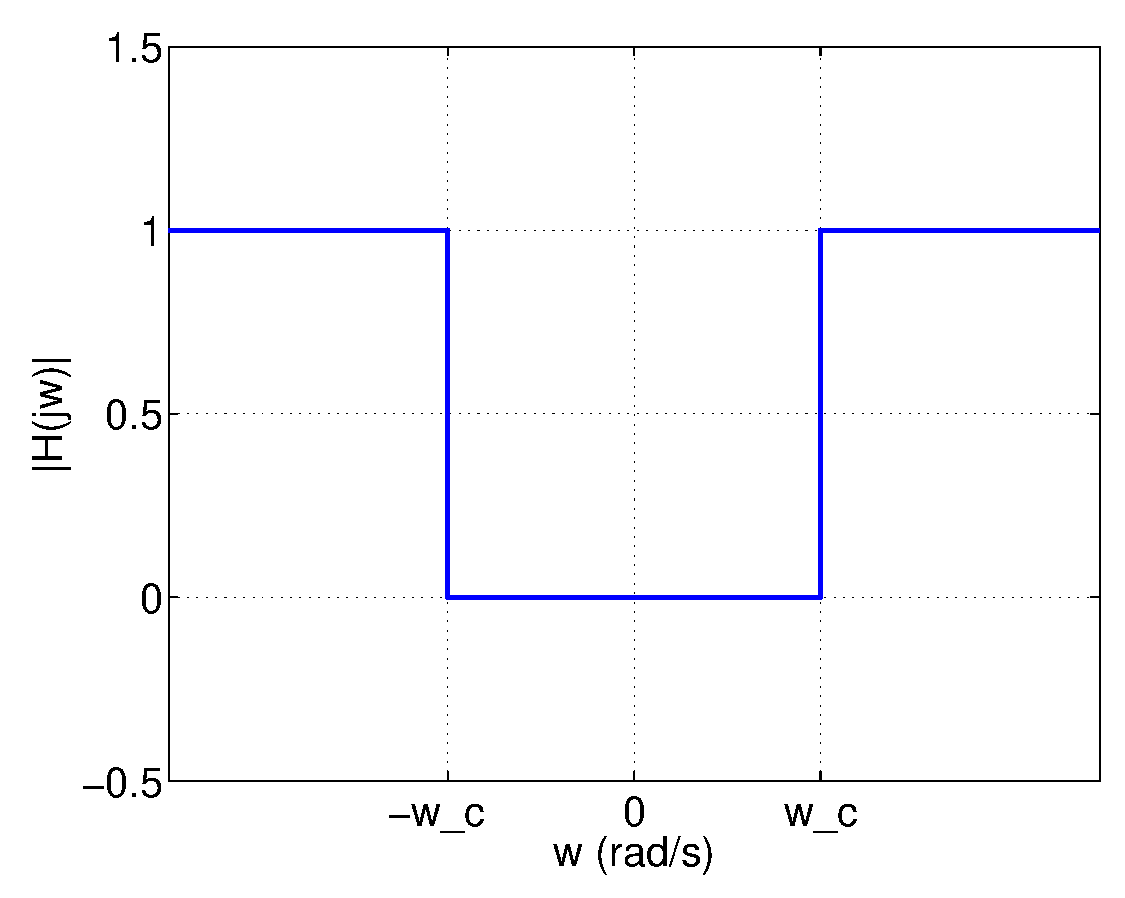
\includegraphics[width=3.2cm]{./Figures/FiltroPAlta.eps}  \end{figure}}

\vspace{-0.2cm}




\end{column}
\begin{column}{5 cm}
\scriptsize
\centering{
Filtro paso banda}

\vspace{0.1cm}


$\scriptsize H(jw)\!=\!\left \{  \!\!\!\begin{array}{l} 1, \:  w_{1}\!\!<\!\!w\!\!<\!\!w_{2}\\0, \:\textrm{c.c.}  \end{array}\right .$

\vspace{-0.4cm}

{\begin{figure} \centering 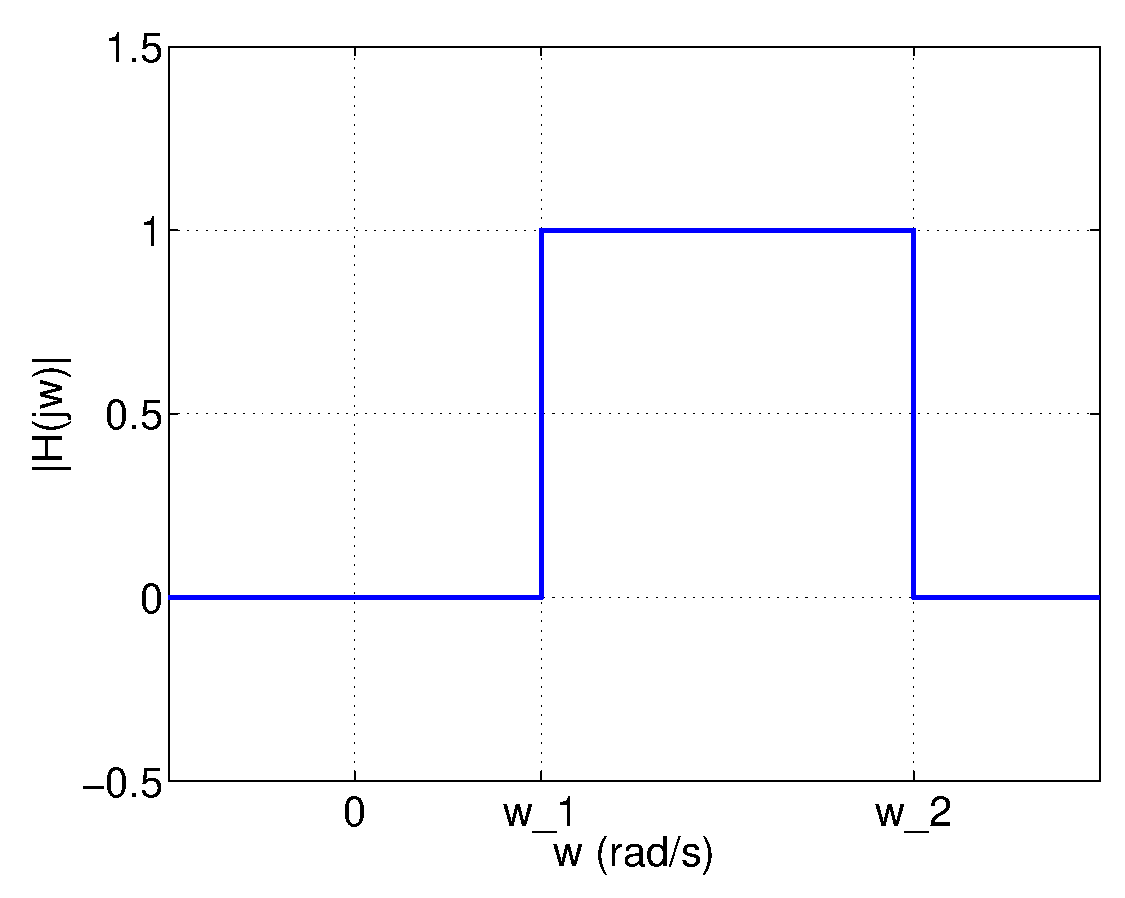
\includegraphics[width=3.2cm]{./Figures/FiltroPBanda.eps}  \end{figure}}

\vspace{-0.2cm}

\centering{
Filtro supresor banda}

\vspace{0.1cm}


$\scriptsize H(jw)\!=\!\left \{  \!\!\!\begin{array}{l} 0, \:  w_{1}\!\!<\!\!w\!\!<\!\!w_{2}\\1, \:\textrm{c.c.}  \end{array}\right .$

\vspace{-0.4cm}

{\begin{figure} \centering 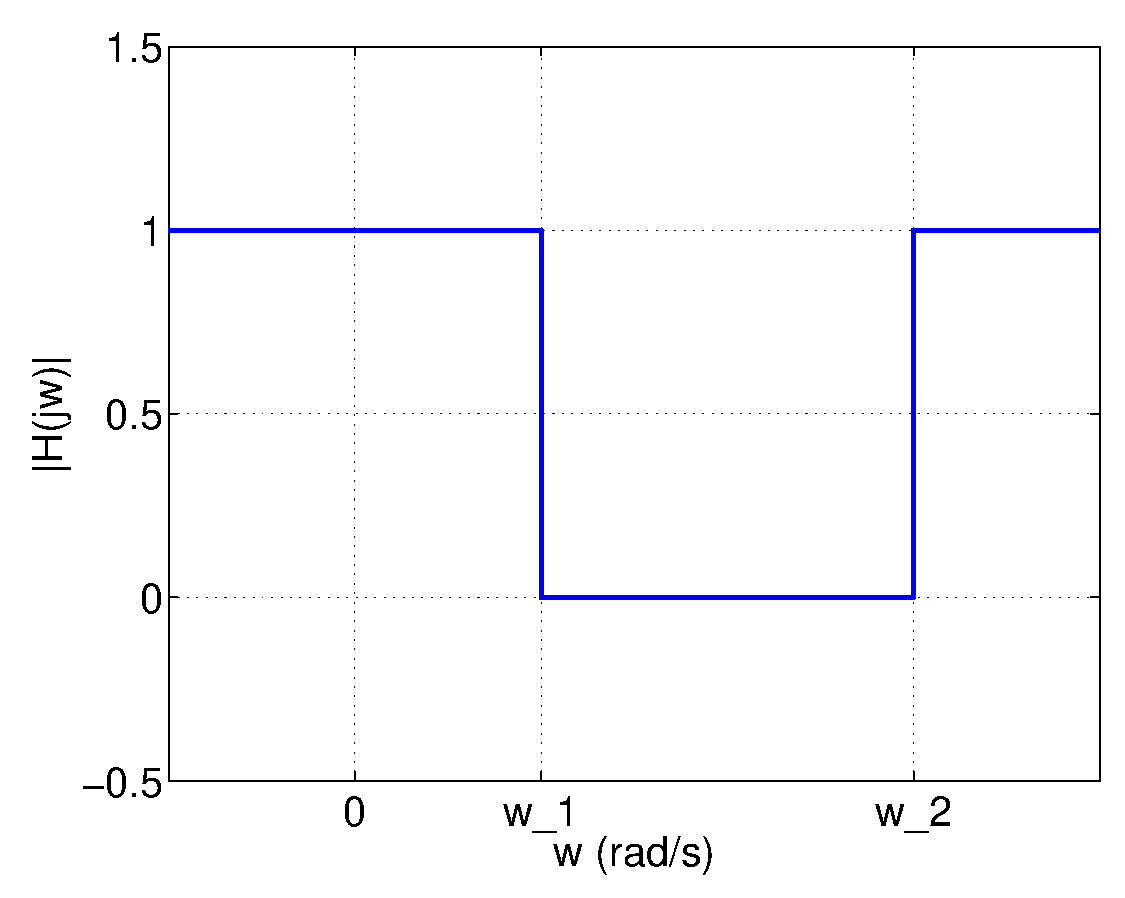
\includegraphics[width=3.2cm]{./Figures/FiltroSBanda.eps}  \end{figure}}

\vspace{-0.2cm}


\end{column}
\end{columns}



\end{frame}